\section{Issues} \label{sec:issues}

\subsection{Zero Probabilities in Learned CPTs}
It was noticed that some of the Conditional Probability Tables (CPT/CPD), that pomegranate learned from the data set (i.e. by solving the problem defined in Subsec. \ref{subsec:bnstructurelearning}), presented entries with $0$ value.

The assignment of the extreme probabilities $1$ and $0$, while perfectly coherent in the frequentist approach, is not in line with the Bayesian one.
This is because of the different conception of probabilities between the two approaches, as discussed in Subsec. \ref{subsec:probability-distributions}.
A frequentist perspective would happily assign probability zero to an event not present in the data set while a Bayesian would refrain to do so, as having a zero or one prior belief makes every posterior, calculated using Bayes' Rule (Eq. \ref{eq:bayes-theorem}), also zero or one.
The necessity to avoid assigning prior probability beliefs of $0$ or $1$, has been named \enquote{Cromwell's Rule} by \cite{Jackman2009}.

It would be an epistemological error to be absolutely sure, one way or another, of any \textit{a posteriori/syntetic proposition} and thus we should refrain from assigning absolute belief or disbelief into their truth value.
This, apart from questions regarding the ontological determinism of Reality, is also against the intended use of statistics, that should be applied in cases of uncertainty and not in those of deterministic mechanism.
We should do so only for \textit{a priori propositions}, for example those referring to Mathematic or Logic, but not for any \textit{a posteriori statements} i.e. those whose truth value is based on experience (for a definition of these see the Introduction of \cite{Kant1998}).

To solve the issue in the context of this work, a simple post-learning correction was applied; specifically a small positive constant was added to every zero-valued entry in the CPTs in pomegranate's model.
The methodologically correct approach would have been to apply \textit{Laplace Smoothing}, a standard technique used to \textit{smooth} categorical data.
The method would entail adding a \textit{pseudocount} $\alpha$ to every empirical probability estimated from the data set; given $x_i$ the count of occurrences of event $i$ a set of $N$ events, the un-smoothed empirical probability is:
\begin{equation}
	p_i = \frac{x_{i}}{N}
\end{equation}
while the smoothed one is given by:
\begin{equation}
	p_i^*=\frac{x_{i}+\alpha}{N+\alpha d}
\end{equation}
with $d$ the number of possible categories.
The value of $\alpha$ should be chosen to reflect any prior knowledge regarding the events; in the case there were none, a non-informative prior should be chosen as stated by the \textit{principle of indifference} (in absence of any evidence one should distribute his beliefs uniformly).
The simplest possible non-informed approach is to increment every event's count in the data set by one, including the ones not appearing.
Thus the relative frequency between events will be maintained but there will be no event $i$ s.t. $x_i=0=p_i$.
Unfortunately implementing this approach, while the most methodologically sound way of proceeding, would have been very time-consuming and outside the main focus of this thesis.
The chosen strategy of adding a small positive constant $\epsilon$ to each empirical probability $p_i$, while not strictly correct, is extremely unlikely to change the learned CPTs.
This can not be ruled out a priori and would necessitate of sensitivity analysis to be settled, but the prior belief is that it is very unlikely to happen.

The applied algorithm, termed \textit{epsilon smoothing}, is based on adding and subtracting \enquote{probability atoms} $\epsilon$ with the objective of removing zeros in the CPTs and maintaining the normalisation, so that the result is still a valid probability distribution (for an introduction, see Subsec. \ref{subsec:probability-distributions}).
We work with probability atoms $\epsilon$ so as not to incur in numerical imprecisions in the implementation, as only additions and subtractions are used.
Every zero-valued element in a CPT column has a quantity $\epsilon \times \#!0$ added to it, with $\#!0$ the number of elements in the distribution that are not zero, and every non-zero entry has $\#0$, the number of zero elements, atoms subtracted from it.
The end result is obviously still a correctly normalised probability distribution because given a probability distribution $P$, with $n$ elements $p$, of which $\#0$ are zero, and the  distribution $P^*$ resulting from to the described procedure:
\begin{align*}
	&\sum_{i=0}^{n} p_i = 1 \\
	\wedge  \quad &1 - \{ \#0 \times [(n - \#0) \times \epsilon] \} + \{ (n - \#0) \times [\#0 \times \epsilon] \}  = 1 \\
	\Rightarrow \quad  &\sum_{i=0}^{n} p^*_i = 1
\end{align*}
The pseudocode is shown in Alg. \ref{alg:epsilon-smoothing}.

\begin{algorithm}[htp!]
	\caption{Epsilon Smoothing algorithm pseudocode}
	\label{alg:epsilon-smoothing}
	\begin{algorithmic}[1]
		\State $\epsilon=$ smallest positive constant
		\For{$s$ in model CPTs}
			\For{$c$ in $s$'s columns} \Comment{distributions of values are organised column-wise}
				\State $num\_zeros$ = number of zero-valued entries in $c$
				\State $num\_non\_zeros$ = $|c|$ - $num\_zeros$
				\For{$v$ in $c$}
					\If{$v$ equal to $0$}
						\State $v += \epsilon \times num\_non\_zeros$
					\Else
						\State $v -= \epsilon \times num\_zeros$
					\EndIf
				\EndFor
			\EndFor
		\EndFor
	\end{algorithmic}
\end{algorithm}

If the procedure were applied to the CPT reproduced in Tab. \ref{tab:rec-cpd-issues}, it would yield the one shown in Tab. \ref{tab:rec-cpd-epsilon}.

\begin{table*}[htbp]
\centering
\caption{\textbf{recettori estrogeni} CPD}
\begin{tabularx}{\textwidth/2}{ccXX}
\toprule
      & &  \multicolumn{2}{c}{\textbf{mut17q21}} \\
\cmidrule(lr){3-4}
 & & 0 & 1    \\ 
 \multirow{3}{*}{\textbf{rec. estr.}}  & 0 & $0.68 - \epsilon$ & 0.13  \\
 & 1 & $0.0 + 2\epsilon$ & 0.02    \\
 & 2 & $0.31 - \epsilon$ & 0.84 \\
\bottomrule
\end{tabularx}
\label{tab:rec-cpd-epsilon}
\end{table*}


\subsection{MPE Calculation}
The main issue encountered during the implementation of the system described in Sec. \ref{sec:implemented-tool}, was that of correctly calculating the MPE.
Initially, an attempt was made to write a custom function \texttt{export\_model\_to\_uai} to generate a UAI file (described in \ref{subsec:libraries}) directly from the pomegranate Bayesian Network model.
This UAI file was fed to DAOOPT to generate the MPE solution as recounted in Subsec. \ref{subsec:algorithms} under the \textbf{MPE Algorithms Comparison} header.
When compared with the MPE solution generated directly using pgmpy's \texttt{map\_query} function, it was seen that these disagreed in almost all cases.
This shouldn't have been the case as both were generated using exact methods: Variable Elimination in pgmpy's case and AND/OR Branch-and-Bound for DAOOPT.

While investigating the cause for this divergence, I came across an undocumented feature of pgmpy: a \texttt{UAIWriter} class that should have converted the pgmpy-based model (that was converted from the pomegranate-based model as recounted in Subsec. \ref{subsec:algorithms} at the \textbf{Pairwise Correlations} header) to the correct UAI file representing it.
When this alternative UAI file was used as input for DAOOPT, the resulting MPE not only diverged from that calculated based on \texttt{export\_model\_to\_uai}, that was to be expected, but also from that calculated directly with pgmpy using \texttt{map\_query}, that was surprising.

The conversion from the pomegranate-based to the pgmpy-based model was thoroughly tested using conditional probability and independencies query, so the issue is most likely to be found elsewhere.
As the DAOOPT MPE solution generated starting from the UAI differs from the one calculated directly with pgmpy, there must be a bug either in pgmpy's UAI exporter or in its inference method.
It is unclear if the following is still an issue (\url{https://github.com/pgmpy/pgmpy/issues/856}) but a series of test on simple networks, where the MPE calculation were carried out manually, seemed to confirm that \texttt{map\_query} was returning the correct MPE solution.

For example, in the small BN whose structure is shown in Fig. \ref{fig:issues-bn} and the CPDs of the nodes in Tab. \ref{tab:mut-cpd-issues}, \ref{tab:eta-cpd-issues}, \ref{tab:rec-cpd-issues} and \ref{tab:diff-cpd-issues}, pgmpy's \texttt{map\_query} and DAOOPT returned different solutions to the following MPE query:
\begin{align*}
  argmax_{x,y,z}\mathbb{P}(
  &\text{differenziazione}=x, \\
  &\text{mut17q21}=y, \\
  &\text{recettori estrogeni}=z | \text{eta arrotondata}=0) \\
\end{align*}
\texttt{map\_query} returned the assignment: 
\begin{align} \label{eq:pgmpy-assignment}
  \text{differenziazione}=1, 
  \text{mut17q21}=1, 
  \text{recettori estrogeni}=2
\end{align}
while DAOOPT returned:
\begin{align} \label{eq:daoopt-assignment}
  \text{differenziazione}=0, 
  \text{mut17q21}=1, 
  \text{recettori estrogeni}=2
\end{align}

In such a small network it is easy to verify that the probability of \ref{eq:pgmpy-assignment} is: $0.99 \times 0.84 \times 0.60 = 0.50$ and that it is the MPE solution; while that of \ref{eq:daoopt-assignment} is $0.99 \times 0.84 \times 0.21 = 0.17$ that makes it obviously incorrect.

\begin{figure}[htbp]
\centerline{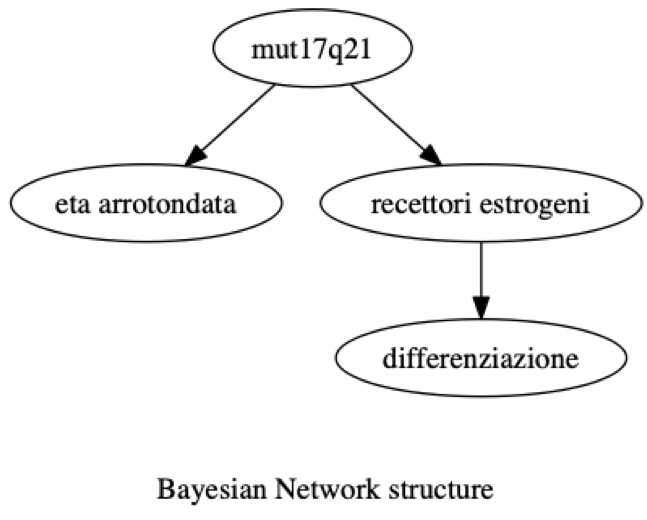
\includegraphics[width=\columnwidth/2]{results/images/issues-bn}}
\caption{Independencies query natural language output.}
\label{fig:issues-bn}
\end{figure}

\begin{table*}[htbp]
\centering
\caption{\textbf{mut17q21} CPD}
\begin{tabularx}{\textwidth/2}{cXX}
\toprule
& 0 & 1    \\ 
\textbf{mut17q21} & 0.006 & 0.99  \\
\bottomrule
\end{tabularx}
\label{tab:mut-cpd-issues}
\end{table*}

\begin{table*}[htbp]
\centering
\caption{\textbf{eta arrotondata} CPD}
\begin{tabularx}{\textwidth/2}{ccXX}
\toprule
      & &  \multicolumn{2}{c}{\textbf{mut17q21}} \\
\cmidrule(lr){3-4}
 & & 0 & 1    \\ 
 \multirow{3}{*}{\textbf{eta arr.}}  & 0 & 0.42 & 0.04  \\
 & 1 & 0.42 & 0.17    \\
 & 2 & 0.15 & 0.78 \\
\bottomrule
\end{tabularx}
\label{tab:eta-cpd-issues}
\end{table*}

\begin{table*}[htbp]
\centering
\caption{\textbf{recettori estrogeni} CPD}
\begin{tabularx}{\textwidth/2}{ccXX}
\toprule
      & &  \multicolumn{2}{c}{\textbf{mut17q21}} \\
\cmidrule(lr){3-4}
 & & 0 & 1    \\ 
 \multirow{3}{*}{\textbf{rec. estr.}}  & 0 & 0.68 & 0.13  \\
 & 1 & 0.0 & 0.02    \\
 & 2 & 0.31 & 0.84 \\
\bottomrule
\end{tabularx}
\label{tab:rec-cpd-issues}
\end{table*}

\begin{table*}[htbp]
\centering
\caption{\textbf{differenziazione} CPD}
\begin{tabularx}{\textwidth/2}{ccXXX}
\toprule
      & &  \multicolumn{3}{c}{\textbf{recettori estr.}} \\
\cmidrule(lr){3-5}
 & & 0 & 1 & 2   \\ 
 \multirow{3}{*}{\textbf{diff.}}  & 0 & 0.012 & 0.16 & 0.21  \\
 & 1 & 0.18 & 0.43 & 0.60    \\
 & 2 & 0.80 & 0.40 & 0.18 \\
\bottomrule
\end{tabularx}
\label{tab:diff-cpd-issues}
\end{table*}
